\documentclass[12pt ,a4paper , twoside , openright ]{book}

\usepackage[a4paper,top=2.5cm,bottom=2.5cm,left=3cm,right=3cm]{geometry}
\usepackage{graphicx}
\usepackage[font={small,it}]{caption}
\usepackage{subcaption}
\usepackage{layouts}
\usepackage{titlesec}
\usepackage[T1]{fontenc}
\usepackage[utf8]{inputenc}
\usepackage{lmodern}
\usepackage{hyperref}
\usepackage[italian]{babel}
\usepackage[usenames]{color} 
\usepackage{graphicx}
\usepackage[bottom]{footmisc}
\graphicspath{ {./images/} }
\definecolor{mygreen}{rgb}{0,0.6,0}
\definecolor{mygray}{rgb}{0.5,0.5,0.5}
\definecolor{mymauve}{rgb}{0.58,0,0.82}
\usepackage{tikz} % for background logo in frontespizio
\addtolength{\skip\footins}{3pc plus 5pt}
\renewcommand{\arraystretch}{1.5}
\pagestyle{plain}
\usepackage{comment}
\usepackage{listingsutf8}
\usepackage{emptypage}
\usepackage[Conny]{fncychap}
\usepackage{minitoc}
\usepackage{natbib}
\bibliographystyle{unsrt} 

\lstset{ 
	backgroundcolor=\color{white}, 
	basicstyle=\tiny\ttfamily,
	breakatwhitespace=false, 
	breaklines=true,
	captionpos=b, 
	commentstyle=\color{mygreen}, 
	escapeinside={\%*}{*)}, 
	extendedchars=true, 
	frame=single,
	keepspaces=true, 
	keywordstyle=\color{blue},
	inputencoding=utf8/latin1,
	morekeywords={*,...}, 
	numbers=left, 
	numbersep=5pt, 
	numberstyle=\tiny\color{mygray}, 
	rulecolor=\color{black}, 
	showspaces=false, 
	showstringspaces=false, 
	showtabs=false, 
	stepnumber=1, 
	stringstyle=\color{mymauve}, 
	tabsize=2, 
}

\definecolor{darkgray}{rgb}{.4,.4,.4}
\definecolor{green}{rgb}{0.65, 0.12, 0.82}

\lstdefinelanguage{JavaScript}{
	keywords={typeof, new, true, false, catch, function, return, null, catch, switch, var, if, in, while, do, else, case, break},
	keywordstyle=\color{blue}\bfseries,
	ndkeywords={class, export, boolean, throw, implements, import, this},
	ndkeywordstyle=\color{darkgray}\bfseries,
	identifierstyle=\color{black},
	sensitive=false,
	comment=[l]{//},
	morecomment=[s]{/*}{*/},
	commentstyle=\color{purple}\ttfamily,
	stringstyle=\color{red}\ttfamily,
	morestring=[b]',
	morestring=[b]"
}

\lstset{
	language=JavaScript,
	extendedchars=true,
	basicstyle=\normalsize\ttfamily,
	showstringspaces=false,
	showspaces=false,
	numbers=left,
	numberstyle=\scriptsize,
	numbersep=8pt,
	tabsize=2,
	breaklines=true,
	showtabs=false,
	captionpos=b
}

\author{
	Daniele Rigon - 857319 \\
}

\pagestyle{plain}
\author{Daniele Rigon}
\title{Web APIs Security}
\makeindex

\begin{document}
	\thispagestyle{empty}
	\begin{tikzpicture}[remember picture,overlay]
	\node[inner sep=0pt,anchor=0,opacity=0.5]{
\includegraphics{CaFoscariLogo.png}};
	\node[inner sep=40pt,anchor=45,opacity=0.5]{Universit\'a};
	\node[inner sep=55pt,anchor=55,opacity=0.5]{Ca' Foscari};
	\node[inner sep=70pt,anchor=56,opacity=0.5]{Venezia};
	\end{tikzpicture}
	\begin{center}
		\vspace*{0.5cm}
		\Large
		\LARGE \textbf{Corso di Laurea }\\
		\LARGE \textbf{in Informatica}\\
		\textit{\large Ordinamento ex D.M. 270/2004}
		
		\vspace*{1cm}
		\Large Tesi di Laurea\\
		
		\vspace*{1cm}
		\LARGE \textbf{Web APIs Security}\\
	\end{center}
	\begin{flushleft}
		\vspace*{2.6cm} \normalsize
		\textbf{Relatore}\\
		Dott. Stefano Calzavara
		
		\vspace*{1.3cm} \normalsize
		\textbf{Correlatore}\\
		Dott. Marco Squarcina
		
		\vspace*{1.3cm} \normalsize
		\textbf{Laureando}\\
		Daniele Rigon \\
		Matricola 857319 \\		
		
		\vspace*{1.3cm} \normalsize
		\textbf{Anno Accademico}\\
		2018/2019 \\	
	\end{flushleft}

	\cleardoublepage
	\thispagestyle{empty}
	\begin{flushright}
		\vspace*{3.0cm}\textit{Alla mia famiglia.}
	\end{flushright}
	\cleardoublepage
	\dominitoc
	\frontmatter
	\pagenumbering{Roman}
	\tableofcontents
	\cleardoublepage
	\mainmatter
	\setcounter{page}{1}
	\chapter{Introduzione}
	Nel corso degli ultimi decenni la tecnologia è diventata sempre più presente nella quotidianità di ogni individuo, che riguardi lavoro, svago o vita quotidiana, e in particolar modo Internet. Come ogni cosa presenta però aspetti positivi e negativi e, essendo il World Wide Web un mondo vastissimo, sono numerosi i rischi al suo interno. \\ 
	In questa tesi ho preso in esame uno strumento molto utilizzato e che probabilmente alcuni di noi ne usufruiscono senza saperlo, le Application Programming Interface (API). Questo strumento, molto diffuso in ambiente informatico, semplifica molto la programmazione. Esso infatti permette di usufruire di informazioni messe a disposizione da terze parti evitando di scrivere da zero i codici, eliminando lavoro non a valore aggiunto oltre ad una correttezza della funzionalità utilizzate oltre a ciò questo insieme di protocolli e procedure rende la comunicazione tra piattaforme diverse molto più semplice. Ogni volta che ci si logga in un sito tramite Google o Facebook, o si utilizzano le mappe di Maps all'interno di pagine Web, o si accede ad un databse durante la compilazione di un form online, stiamo utilizzando le API. Pensando più in grande le API si utilizzano anche nell'intelligenza artificiale, come servizi di \textit{chatbot}\footnote{Assistenti virtuali disponibili 24/7 capaci di dare risposte in tempo reale.}, nell'\textit{Internet of Things (IoT)}\footnote{Internet applicato al mondo concreto, come smarthouse, industria 4.0, ecc.} e nel \textit{Machine Learning}\footnote{Ramo dell'intelligenza artificiale che studia e crea algoritmi che apprendano informazioni da un insieme di dati in modo da crearne delle previsioni.}. Tutto ciò porta anche ad una esperienza utente più intuitiva e di facile apprendimento. \\
	La tesi è articolata in tre capitoli. Il primo esplica la \textit{Geolocation API}\cite{rif2} utile a tracciare la posizione all'interno di un sito web o un'applicazione online. Nel secondo è spiegata \textit{PaymentRequest API}\cite{rif1} la quale, salvando le informazioni imputate, permette la riutilizzazione di essere senza il reinserimento manuale Nel terzo ed ultimo capitolo l'attenzione verte sui \textit{Service Worker}\cite{rif5}, usati principalmente nelle \textit{Progressive Web App}\footnote{Appicazioni presenti sulle pagine web che si comportano come applicazioni native.} ai fini di miglioramento dell'esperienza utente.
	\\
	Tutte le informazioni presenti nella tesi sono reperibili al seguente repository GitHub: \url{https://github.com/danielerigon4/Tesi-Web-Api}.
	\cleardoublepage
	
	\chapter{Geolocation API}
	\section{Overview}
	La Geolocation API viene utilizzata per ottenere la posizione geografica di un utente. 
	Poiché questo può compromettere la privacy, la posizione non è disponibile a meno che l'utente non la approvi: in un dispositivo mobile si usano le coordinate provenienti dal sensore GPS, mentre in un computer l'indirizzo IP.
	\section{Metodi}
	Nella Geolocation API la posizione viene resa nota tramite la proprietà \textit{navigator.geolocation}\cite{rif4} dell'oggetto \textit{Navigator}, la quale possiede esclusivamente tre metodi: \textit{getCurrentPosition}, \textit{watchPosition} e \textit{clearWatch}. I primi due restituiscono la posizione corrente, mentre il terzo annulla la ricerca. La differenza tra \textit{getCurrentPosition} e \textit{watchPosition} è insita nella loro periodicità: se il primo metodo fornisce il dato una sola volta, il secondo lo comunica automaticamente a intervalli di tempo fissati o ogni qualvolta la posizione cambi. Va specificato che \textit{getCurrentPosition} è pensata per restituire la posizione nel più breve tempo possibile, avendo quindi una bassa precisione. Da notare che \textit{clearWatch} può essere utilizzato solamente se in precedenza uno dei due metodi è stato avviato, quindi se esiste una posizione. \\
	La sintassi per invocare tali metodi si può vedere nel codice 2.1.
	\lstinputlisting[caption= Geolocation API - Sintassi dei metodi\cite{rif4}]{code/Sintassi.js} 
	E' possibile distinguere tre parametri della funzione per \textit{getCurrentPosition} e \textit{watchPosition}.
	La \textit{SuccessCallback}, parametro obbligatorio, viene rischiesta quando la chiamata a una nuova posizione va a buon fine. \textit{ErrorCallback} e  \textit{Opzioni}, invocate rispettivamente per gestire la presenza di uno o più errori e definire i parametri delle chiamate alle due callback, sono invece parametri opzionali.
	\newpage
	\section{Esempio di implementazione}
	Supponiamo di avere la pagina di esempio della Figura 2.1, dove poter osservare il funzionamento dei tre metodi descritti precedentemente eseguendoli tramite tre pulsanti presenti nella pagina, denominati per semplicità con la medesima azione che richiamiamo\cite{rif8}. All'inizio, non essendo ancora stata invocata nessuna funzione, l'interfaccia restituisce l'indisponibilità del dato. Quando invece si selezionerà una delle azioni presenti nella pagina, le voci "unavailable" saranno popolate dalle informazioni riguardanti le geolocalizzazione fornite dopo l'accetazione del trattamento di queste da parte dell'utente. Se l'utente non acconsente nel menù Log comparirà un messaggio di errore, come mostrato in Figura 2.3.
	\begin{figure}[h]
		\centering
		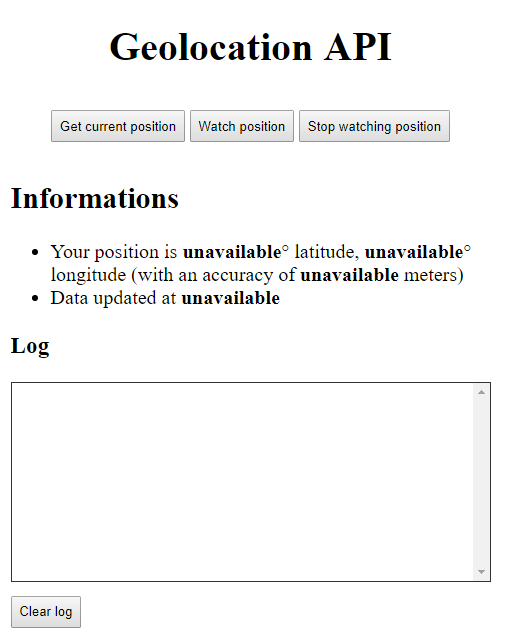
\includegraphics[width=0.5\linewidth]{geo1}
		\caption{Geolocation API - Implementazione pagina d'esempio\cite{rif8}}
		\label{fig: Geolocation API - Implementazione pagina d'esempio}
	\end{figure}
	\\
	L'invocazione avviene tramite un \textit{addEventListener}, ovvero un metodo che associa un insieme di eventi ad ogni elemento specificato nel \textit{Document Object Model (DOM)}\footnote{API standardizzata da W3C per accedere e modificare gli elementi di una pagina web.}.	
	\pagebreak
	\lstinputlisting[firstline=26,lastline=36,caption= Geolocation API - Invocazione dei metodi della Geolocation tramite AddEventListener \cite{rif8}]{code/EsempioCompleto.js} 
	Tale evento farà comparire una finestra di richiesta posizione, la quale porterà a due differenti scenari nel caso l'utente accetti o meno.
	\begin{figure}[h]
		\centering
		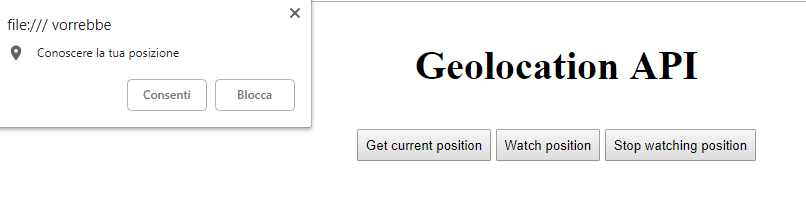
\includegraphics[width=0.8\linewidth]{geo2}
		\caption{Geolocation API - Richiesta permesso posizione\cite{rif8}}
		\label{fig: Geolocation API - Richiesta permesso posizione}
	\end{figure} \\
	Se l'utente rifiuta la concessione alla determinazione della posizione, questa non è calcolata. Viene richiamata la funzione di \textit{ErrorCallback} e visualizzato un messaggio di errore postato in Figura 2.3.
	\begin{figure}[h]
		\centering
		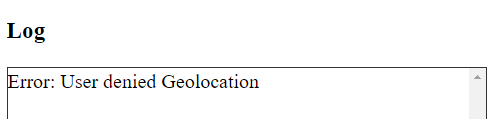
\includegraphics[width=0.8\linewidth]{geo3}
		\caption{Geolocation API - Rifiuto autorizzazione\cite{rif8}}
		\label{fig: Geolocation API - Rifiuto autorizzazione}
	\end{figure} \\
	Viceversa, se l'utente acconsente, la chiamata alla funzione \textit{SuccessCallback} andrà a buon fine e compariranno tutte le informazioni disponibili ricavate tramite \textit{getElementById}\footnote{Ogni elemento della pagina può essere associato a un ID univoco in modo da accedervi velocemente}, come raffigurato nella Figura 2.4.
	\lstinputlisting[firstline=11,lastline=16,caption= Geolocation API - Informazioni della pagina tramite getElementById\cite{rif8}]{code/EsempioCompleto.js}
	\begin{figure}[h]
	 	\centering
	 	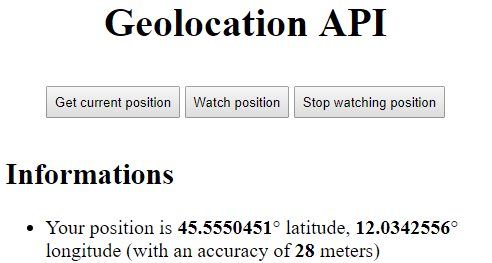
\includegraphics[width=0.5\linewidth]{geo4}
	 	\caption{Geolocation API - Accettazione autorizzazione\cite{rif8}}
	 	\label{fig: Geolocation API - Accettazione autorizzazione}
	\end{figure}
	\section{Rischi e sicurezza} 
	Ognuno di noi ogni giorno, consapevolmente o meno, condivide la propria posizione più e più volte. Ce ne accorgiamo quando utilizziamo applicazioni di fitness che tracciano i nostri percorsi o quando impostiamo il navigatore verso una destinazione. Succede però che ci compaiano delle notifiche nelle quali il cellulare ci chiede di impostare certe destinazioni frequenti come luoghi di interesse, o addirittura ci propone orari di partenza casa - lavoro per trovare meno traffico. Così come possiamo ricercare una foto tramite geo tag invece di scorrere album interi. Tutto ciò è reso possibile da questa API. Viene spontaneo chiederci dove vadano questi dati, se sono tenuti al sicuro e soprattutto se possono essere rubati. Le norme sulla privacy e sulla condivisione dei dati prevedono che le informazioni personali delle applicazioni siano caricate dal cellulare ai server tramite una connessione sicura che deve essere crittografata, e tali dati non possono essere ceduti a terze parti senza il consenso del diretto interessato. Tuttavia nulla è garantito totalmente. \\
	Possono esserci infatti differenti modi per rubare informazioni sensibili, due dei quali vengono presi in analisi. \\
	Una possibilità è data dal fatto che l'utente accetti di condividere la propria posizione all'interno di un sito malevolo, ignaro del fatto che tale indirizzo non sia sicuro. \\
	Un'altra modalità di attacco, più diffusa rispetto alla precedente, avviene attraverso un \textit{Cross-Site Scripting(XSS)}. Si tratta di una falla delle applicazioni web che provoca l'inserimento e l'esecuzione di script lato client permettendo la visualizzazione, raccolta e  manipolazione di dati, oltre alla modifica delle pagine web. Tale tipo di vulnerabilità è di due tipi: persistente e non \cite{rif28}. Il Cross-Site Scripting non persistente è sfruttato prettamente nelle pagine web senza forme di controllo mentre l'attacco XSS persistente avviene quando i dati forniti vengono conservati in un server, o un database, restando visibili. Per capire meglio la differenza pensiamo a due esempi. Quando si compilano i campi di un form online e i dati vengono inviati si è nel primo caso. Si supponga invece di essere iscritti ad un sito; in questo caso informazioni come nome, cognome e mail sono salvati in un server, ma nascoste agli utenti. Un possibile attaccante può rubare tali informazioni inserendo uno script progettato in modo tale che, quando il proprio profilo viene visitato, o qualcunque azione sia associata a tale script, il browser lo elabori in modo da rubare le informazioni sensibili degli altri utenti. Prendendo questo esempio, dato che latitudine e longitudine, utili a tracciare le coordinate dell'utente, risiedono all'interno del \textit{DOM}, ci troviamo nella situazione sopra descritta. All'apertura di una pagina all'interno di un sito web potrebbe comparire una finestra come quella in Figura 2.2. Questa potrebbe essere collegata ad uno script \cite{rif7} in grado di salvare \textit{coords.latitude} e \textit{coords.langitude}, transitanti nel DOM, memorizzandole in una variabile. Se l'utente non disabilita il tracciamento della posizione, che rimarrà esposta, si ha un attacco XSS persistente. Si veda, a titolo di esempio, lo script 2.4 in grado di effettuare questo tipo di attacco.
	\lstinputlisting[caption= Geolocation API - Script in grado di rubare informazioni sensibili dell'utente\cite{rif7}]{code/script.js}
	\pagebreak
	\section{Conclusioni}
	In questo capitolo si sono analizzate le specifiche, i vantaggi e i problemi di questa API. Ci si rende conto come ognuno di noi ogni giorno, anche senza saperlo, utilizzi questo strumento, avendone molti vantaggi. Uno sportivo può tenere traccia dei percorsi di allenamento, un rappresentante degli itinerari lavorativi, un corriere delle consegne fatte e previste e chiunque può ritrovare il proprio smartphone smarrito. Oggigiorno, anche grazie alla connessione continua con questi strumenti, l'utilizzo diviene indispensabile per coodotà e velocità che soddisfano molte esigenze in un mondo ormai sempre più dinamico. Nell'era dell'industria 4.0, ogni azienda addotta soluzioni tecnologiche per l'automatizzazione dei processi verso il futuro portando, a volte incosapevolmente, all'aumento del rischio di tutela della privacy personale anche dei dipendenti nel caso avvenga una sottrazione di dati. In ultima analisi ci possono essere anche dei problemi legati alla sicurezza personale. \`E stato detto che i moderni software sono in grado di identificare il luogo presente e futuro di un individuo grazie all'intersecazione di informazioni di geolocalizzazione con quelle personali. Questo può facilitare la possibilità di danni a cose, persone e/o proprietà (furto, stalking, rapimento, violenza domestica, furto d'identità, ecc) oltre alla sottrazione di informazioni personali (indirizzo di casa, lavoro, scuola, itinerari giornalieri, ecc) non solo individuali. \\
	Ci si può difendere utilizzando dei comportamenti idonei a garantire la sicurezza delle nostre informazioni. Come fa già la maggiorparte delle persone, installare un buon antivirus ed evitare siti e mail che non riteniamo sicure sono un buon punto d'inizio. Connettersi ad una rete aperta è uno dei modi più semplici, per un hacker, di rubare dati. Chiunque, tramite la creazione di un hotspot Wi-fi, può rendere credibile il nome della propria rete monitorando ogni accesso. Un altro errore di uso comune è non cambiare le password periodicamente, o peggio usare la stessa password per la maggior parte dei servizi che utilizziamo. \\
	Entrando più nel dettaglio si può salvaguardare ancora di più la propria sicurezza utilizzando browser alternativi ai più comuni, alcuni dei quali pensati apposta a questo scopo, come SRWIron o TorBrowser. Supponendo di non voler cambiare il proprio browser, per comodità o abitudine, si può fare uso delle estensioni (oltre a quelle offerte da antivirus, come Norton Security), come Disconnect, Ghostery, HTTPS Everywhere. Un altro comportamento importante per la salvaguardia dei dati è la navigazione in pagine crittografate, ovvero quello nella forma \textit{https://} invece che \textit{http://}. Oltre ai browser, anche la scelta del motore di ricerca è fondamentale. Infine, dato che un \textit{Internet Service Provider (ISP)}\footnote{Organizzazione che offre, tramite la stipulazione di un contratto, servizi Internet ai propri utenti.} può monitorare tutto ciò che un utente fa in rete, l'uso di una \textit{Virtual Private Network (VPN)}\footnote{Rete Internet privata, nella quale servono delle credenziali per poter accedere, dove ogni trasferimento è criptato.}.
	\cleardoublepage
	\chapter{Payment Request API}
	\section{Overview}
	La \textit{PaymentRequest API}\cite{rif9} nasce con l'intento di semplificare i pagamenti online. Ogni sito web ha il proprio sistema di pagamento e molti richiedono la ridigitazione manuale più volte delle stesse informazioni che potrebbero invece essere memorizzate e riutilizzate dall'API stessa per completare più rapidamente le transazioni online. \\
	I vantaggi sono molteplici\cite{rif13} e interessano aspetti differenti che vanno da una maggior rapidità nell'acquisto a una gestione delle informazioni più veloce e intuitiva. Chiunque utilizzi l'API può gestire i propri dati direttamente dal browser (carte di credito, indirizzi di spedizione, ecc.) e avere tutte queste informazioni sincronizzate così da potervi accedere da ogni dispositivo. Il browser, inoltre, è in grado di verificare la validità delle carte, di comunicare se ce ne sono di scadute (o in prossimità di scadenza) e di suggerire quale di queste utilizzare. In base alle esigenze è possibile anche impostare carte predefinite.
	\section{Metodi}
	Il costruttore \textit{PaymentRequest} ha bisogno di diverse informazioni per poter costruire la richiesta di pagamento. \textit{PaymentMethodData}\cite{rif11} rappresenta l'elenco dei metodi di pagamento accettati, \textit{PaymentDetails}\cite{rif14} delinea i dettagli della transazione (costi, servizi, opzioni di spedizione, ecc.) mentre \textit{PaymentOptions}\cite{rif16} fornisce le informazioni sulla consegna del prodotto (indirizzo fisico, e-mail, ecc.). Dopo aver raccolto tutti questi dati è possibile costruire l'oggetto \textit{PaymentRequest}. Una cosa importante da specificare è che il metodo \textit{show()}\cite{rif12} garantisce la visualizzazione singola dell'interfaccia di pagamento, in modo da non portare l'utilizzatore a commettere errori. Provando ad aprire più di una finestra sarà visualizzato un messaggio di errore, come mostrato in Figura 3.1.
	\begin{figure}[h]
		\centering
		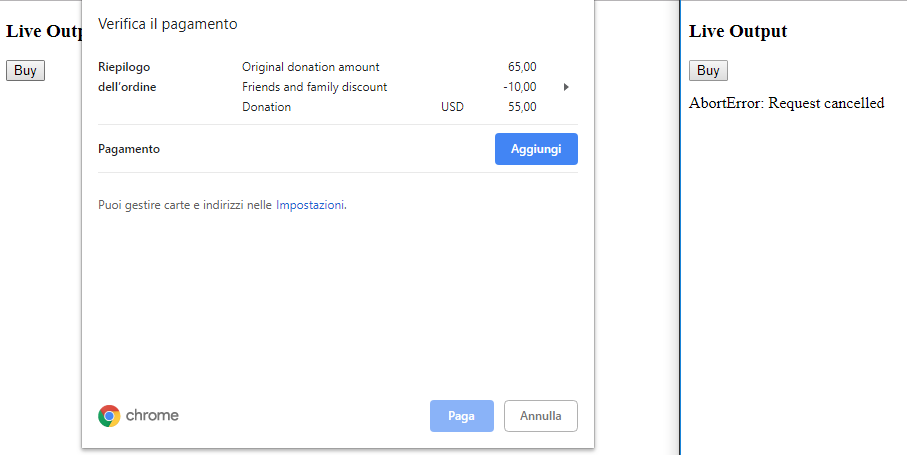
\includegraphics[width=0.8\linewidth]{Buy}
		\caption{PaymentRequest API - Messaggio di errore generato dal metodo show() \cite{rif12}}
		\label{fig: PaymentRequest API - Messaggio di errore generato dal metodo show()}
	\end{figure} \\
	\section{Esempio di implementazione}
	Supponiamo di aver creato l'oggetto \textit{PaymentRequest} contenente, come descritto nel paragrafo precedente, \textit{MethodData}, \textit{Details} e \textit{Options}. 
	\lstinputlisting[caption= PaymentRequest API - Costruzione oggetto PaymentRequest\cite{rif16}]{code/Costruttore.js}
	Una volta codificato esso sarà visualizzabile tramite la chiamata al metodo \textit{request.show()} dove potranno essere inserite le informazioni di pagamento, l'indirizzo di spedizione e una serie di altri campi in base a come è stato costruito l'oggetto (Figura 3.2). Quando tutti i campi saranno compilati e si selezionerà il tasto "paga" sarà creata la \textit{promise}, che potrà avere esito positivo o negativo. In caso di esito positivo verrà soddisfatta la promise e saranno consegnate al commerciante tutte le informazioni inserite dall'acquirente, cosicchè possano essere elaborate sul back-end. Viceversa, in caso di esito negativo, l'operazione di pagamento non andrà a buon fine e comparirà un messaggio di errore che inviterà l'utente a modificare le credenziali, reindirizzandolo alla pagina precedente.
	\begin{figure}[h]
		\centering
		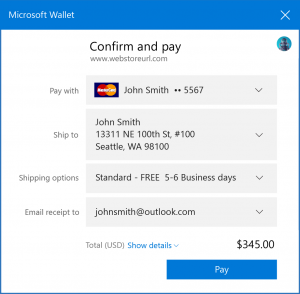
\includegraphics[width=0.5\linewidth]{wallet1}
		\caption{PaymentRequest API - Inserimento credenziali da parte dell'utente\cite{rif30}}
		\label{fig: PaymentRequest API - Inserimento credenziali da parte dell'utente}
	\end{figure} 
	\section{Rischi e sicurezza} 
	Più o meno ogni sito a cui accediamo al giorno d'oggi ha un'area riservata in cui creare il proprio profilo utente, costringendoci a ricordare le credenziali di ognuno di essi, che per comodità tendiamo a far memorizzare al browser.  
	La \textit{PaymentRequest API} cerca di garantire la sicurezza dei dati sensibili attraverso alcune scelte implementative\cite{rif19}. Una di queste è riguardante il metodo \textit{show()}. Oltre a quanto detto, l'API richiede inoltre che esso venga attivato solo tramite la volontà da parte dell'utente, ad esempio con un clic. Tale API, per garantirne la sicurezza, opera solamente in contesti sicuri HTTPS\footnote{HyperText Transfer Protocol over Secure Socket Layer, un protocollo che garantisce una comunicazione in rete sicura attraverso una rete di computer su Internet}. Inoltre, i commercianti possono delegare la memorizzazione delle informazioni a fornitori di servizi di pagamento o al browser, senza avere a carico informazioni sensibili dell'utente. Questo li solleva da responsabilità importanti poichè l'API non supporta direttamente la crittografia dei campi dati. \\
	Come per la precedente API, anche in questa vi sono differenti possibilità di attacco. Un modo per rubare informazioni è il \textit{phishing}. Esso è una truffa che vive all'interno di Internet attraverso la quale sono inserite informazioni personali in pagine che, fingendosi affidabili e autorevoli, non lo sono. Nella maggior parte dei casi inizia con banner pubblicitari, messaggi in social network e, la quasi totalità delle volte, con una mail. Il messaggio ricevuto si presenta come richiesta di apertura di un link da parte di enti, banche o conoscenti, che rimanda a pagine falsamente reali nelle quali inserire i propri dati. Esiste anche una modalità più aggressiva di phishing. Allo stesso modo di come già descritto viene mandata una mail, o un messaggio, apparentemente reale, contenente file .exe invece di indirizzi URL. Tali file sono virus che, una volta eseguiti, si diffondono all'interno del pc, carpendo informazioni in base a come sono costruiti. Simuliamo anche qui, come nella precedente API, un attacco XSS mediante l'inserimento di script dannosi all'interno di una pagina web. Supponiamo di navigare all'interno di un sito affidabile e presumiamo di essere in una pagina di pagamento, come il carrello di Amazon o un'inserzione su Facebook. Inserendo uno script in una di queste pagine, quando il consumatore cliccherà sulla voce di pagamento, sarà eseguito tale script invece di quello del sito. L'utente inserirà tutte le informazioni necessarie al pagamento, convinto di essere sulla pagina sicura ma, al contrario, queste saranno mandate e/o visualizzate dall'attaccante.
	\begin{figure}[h]
		\centering
		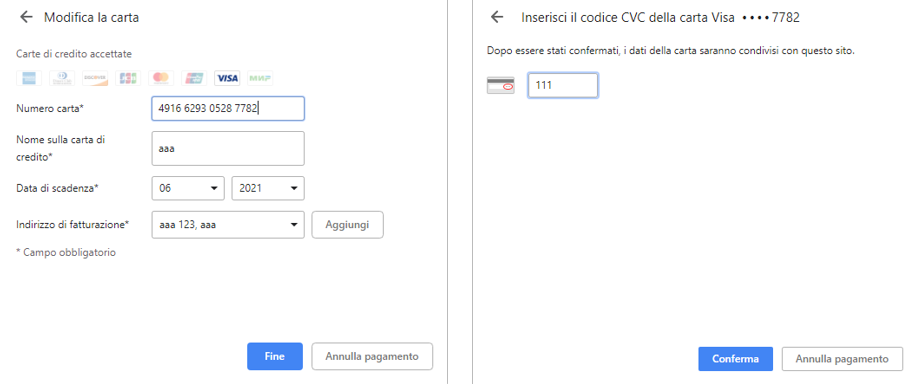
\includegraphics[width=\linewidth]{AttaccoXSS}
		\caption{PaymentRequest API - Attacco XSS\cite{rif30}}
		\label{fig: PaymentRequest API - Attacco XSS}
	\end{figure} 
	\newpage
	Alla richiesta di avvio di un processo di pagamento, ovvero dopo la chiamata al metodo \textit{show()}, è creato l'oggetto \textit{PaymentRequest} nel quale sono inseriti tutti i dati dall'utente. Tale oggetto passa però attraverso il DOM e può quindi essere intercettato e visualizzato. Ad esempio nel campo \textit{details.cardNumber} si può leggere il numero di carta di credito, mentre in \textit{details.cardSecurityCode} si può leggere il codice CVV, come mostrato nella figura successiva.
	\begin{figure}[h]
		\centering
		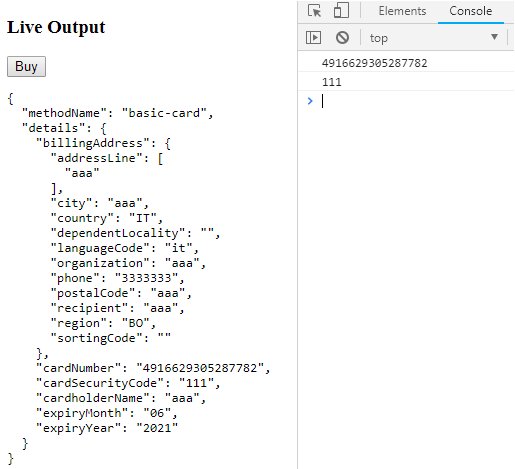
\includegraphics[width=0.8\linewidth]{Informazioni}
		\caption{PaymentRequest API - Informazioni rubate}
		\label{fig: PaymentRequest API - Informazioni rubate}
	\end{figure} 
	\section{Conclusioni}
	\'E facile pensare come ognuno di noi utilizzi tutti i giorni gli strumenti descritti in questo capitolo per acquisti su molti siti di e-commerce. Lo si fa talmente tanto spesso che non si presta più attenzione al fatto che il sito in cui inseriamo i nostri dati sia sicuro o meno, dimenticandoci che per quanto possa essere costruito bene, non sarà immune a vulerabilità e problemi. I vantaggi derivanti dall'uso di queste APIs sono molteplici, perciò è fondamentale attuare comportamenti alla portata di tutti atti a prevenire possibili danni, per poter beneficiare di questi strumenti. Per quanto riguarda la prevenzione agli attacchi XSS, questa informazione è stata descritta ampiamente nelle conclusioni del capitolo precedente. Contro il phishing vi sono alcune attività che possono sembrare banali, ma è meglio ribadirle: non aprire mail o documenti da origini sconosciute, non rivelare le proprie password, aggiornare sempre antivirus e browser applicando le patch di sicurezza\footnote{Aggiornamenti contenenti correzioni di vulnerabilità riscontrate. La maggior parte ha cadenza mensile.}. \'E sempre buona norma, inoltre, verificare l'indirizzo URL della pagina, innanzitutto verificando sia HTTPS, oltre ad assicurarsi non sia una copia del sito originale (ad esempio se sappiamo che il dominio di un certo sito risulta essere .gov e notiamo avere .it allora qualcosa non va).  
	\chapter{Service Worker}
	\section{Overview}
	Un Service Worker\cite{rif25} è uno script Javascript, avviato in background dal browser, utilizzato per aumentare le performance delle applicaziomi web. Esso si trova tra l'applicazione Web e la rete e, similmente ad un \textit{server proxy}\footnote{Intermediario tra web client e ricerca in altri server.}, può intercettare tutte le richieste passanti attraverso di lui agendo secondo regole decise in fase di creazione\cite{rif24}.
	\begin{figure}[h]
		\centering
		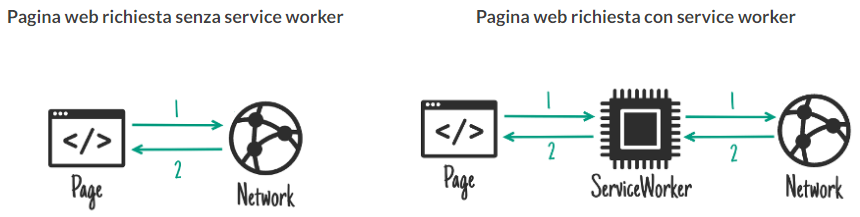
\includegraphics[width=\linewidth]{PaginaSW}
		\caption{Sevice Worker API - Utilizzo Service Worker in una pagina web\cite{rif24}}
		\label{Sevice Worker API - Utilizzo Service Worker in una pagina web}
	\end{figure} \\
	Questo script, essendo separato dalla pagina, non può modificarne gli elementi e può comunicare con essi solamente attraverso le \textit{Promises}\footnote{In Javascript le funzioni, per aspettarsi l'un l'altra, fanno uso delle callback ma, se le funzioni sono molteplici, il codice può diventare lungo e di difficile comprensione. Utilizzando le promise le funzioni eseguiranno i pezzi di codice corrispondenti, in base al fatto che la promise sia stata mantenuta o meno.}: ogni operazione è eseguita asincronicamente e gli elementi del DOM possono essere manipolati solo tramite messaggi. Tale strumento migliora l'esperienza utente grazie a più funzionalità: l'aggiornamento  delle risorse risiedenti nel server, la sincronizzazione dei dati in background, la prelettura delle risorse che serviranno all'utente nel prossimo futuro. In tutto ciò, è il browser a decidere quando il Service Worker sarà o meno in esecuzione. Da notare che, per evitare attacchi \textit{man-in-the-middle}\footnote{Attacco informatico in cui viene alterata la comunicazione tra due parti interessate che credono di comunicare direttamente tra di loro.}, i Service Worker operano esclusivamente in ambienti HTTPS. 
	
	\section{Ciclo di vita di un Service Worker}
	Il ciclo di vita di un Service Worker\cite{rif20, rif21, rif26} è composto da quattro fasi successive che si articolano a partire dalla Registrazione, passando per l'Installazione, l'Attivazione e concludendosi con il Fetch. \\
	La fase di \textit{Registrazione} avviene solamente dopo aver comunicato al browser l'esistenza di un Service Worker all'interno della pagina. La registrazione si realizza mediante il metodo \textit{ServiceWorker.register()} inserendo in tutte le pagine coinvolte uno script simile a quello sotto riportato. Il codice inizia con il controllo, da parte del browser, della presenza del metodo \textit{navigator.serviceWorker}: se supportato, il Service Worker viene registrato correttamente con \textit{navigator.serviceWorker.register} restituendo una Promise. Dato che i Service Worker operano solo in ambienti sicuri, analogamente a quanto visto per la \textit{Payment Request API}, se l'applicazione non è in HTTPS essi non vengono registrati.
	\lstinputlisting[caption=Service Worker API - Registrazione di un Service Worker\cite{rif24}]{code/Registrazione.js}
	Nella fase di \textit{Installazione} il Service Worker viene scaricato e installato al primo accesso ad una pagina. Sarà poi scaricato periodicamente ad intervalli di tempo fissati; se il nuovo file risulta differente da un Service Worker esistente, la nuova versione sarà installata in background ma l'attivazione avverrà quando non ci saranno più pagine che stanno ancora utilizzando il vecchio servizio. \\
	Una volta installato, il Service Worker passa alla fase di \textit{Attivazione} nella quale può controllare gli eventi generati dal client. Possono esistere differenti Service Worker che saranno aggiornati e sostituiti, ma solamente un Service Worker per volta potrà essere eseguito all'interno dello stesso contesto. \'E compito dell'evento \textit{activate} svuotare la cache obsoleta delle versioni precedenti. Una volta che il Service Worker è installato e non sono presenti residui dei Service Worker precedenti, esso potrà effettuare il fetching di risorse restando in attesa di eventuali eventi. \\
	L'ultima fase, relativa all'esperienza utente, è quella di \textit{Fetch}, ovvero l'intercettazione da parte del Service Worker di ogni evento generato dal client, rispondendo alle esigenze secondo le differenti strategie di caching. 
	\section{Rischi e sicurezza}
	I Service Worker, pur operando solo in contesti protetti, non sono privi di limiti legati alla sicurezza\cite{rif29,rif27}. Un Service Worker infatti può importare script da qualsiasi altra origine tramite il metodo \textit{importScripts}. Per mitigare rischi il browser richiede che l'URL di registrazione del Service Worker provenga dalla stessa origine dei propri chiamanti (\textit{https://example.com} è diverso da \textit{https://example.evil.com}). Per questo motivo, per registrare un Service Worker malevolo attraverso questo tipo di attacco, il malintezionato ha bisogno di ospitare i propri script sul server. Considerando una situazione di attacco XSS, quindi con l'inserimento di script all'interno della pagina al fine di rubare dati sensibili, c'è la garanzia che dopo 24 ore la minaccia cesserà di esistere essendo questo il tempo limite di vita di un Service Worker (o meno in base alle regole della pagina). Tale rischio potrebbe quindi essere ulteriormente mitigato con una breve vita dei Service Worker, in modo ragionevole da permettere tuttavia che ne siano sfruttate le potenzialità. Si nota che questo strumento, utilizzato per la velocizzazione e il miglioramento dei tempi di risposta delle applicazioni, potrebbe essere programmato per comportarsi similmente a \textit{man-in-the-middle}, intercettando e modificando i messaggi che intercetta. \\
	Si supponga di avere una pagina HTML che registra un Service Worker attraverso uno script (nell'esempio sottostante è \textit{script.js} a riga 2) il quale intercetta ogni richiesta transitante nella pagina. 
	\lstinputlisting[caption= Service Worker API - Registrazione e installazione Service Worker\cite{rif24}]{code/index.html}
	Una volta completata la registrazione, il Service Worker sarà installato (Nel codice 4.2 tramite il file \textit{install.js}).
	\lstinputlisting[caption=Service Worker API -  Intercettazione di ogni richiesta da parte del Service Worker]{code/install.js}
	In questo esempio compare a video il messaggio di minaccia (Figura 4.2), ma in una situazione ordinaria, una possibile vittima non saprà che le informazioni transitanti nella pagina gli stanno venendo sottratte. 
	Finchè il Service Worker non sarà disinstallato e non verrà cancellata la cache, ogni richiesta verrà intercettata.
	\begin{figure}[h]
		\centering
		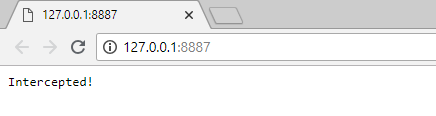
\includegraphics[width=0.7\linewidth]{Intercepted}
		\caption{Service Worker API - Intercettazione di ogni richiesta da parte del Service Worker}
		\label{fig: Service Worker API - Intercettazione di ogni richiesta da parte del Service Worker}
	\end{figure}
	\section{Conclusioni}
	Alla fine di questo capitolo si è capito come molti strumenti, anche molto potenti come i Service Worker, pensati originariamente a scopo positivo, possano essere usati malamente. \\
	Vi sono indubbiamente molteplici vantaggi. Se sfruttati per la caching la navigazione all'interno delle applicazioni diventa molto veloce. Un'altra funzionalità è la sincronizzazione in background delle pagine web consentendo la visualizzazione istantanea dei cambiamenti. I Service Worker permettono anche azioni adeguate in base al contesto, ovvero in assenza o presenza della rete. La rivoluzione maggiore, a mio parere, è la possibilità di inviare notifiche push tramite le web app, diminuendo ulteriormente il divario tra applicazioni online e native. Questo è reso possibile grazie a due strumenti complementari tra loro: la \textit{Push API} e la \textit{Notification API}. La prima segnala la presenza di una notifica mentre la seconda attiva la visualizzazione. Purtroppo gli utenti Apple non possono ancora usufruire di queste tecnologia in quando il browser Safari non è ancora compatibile. \\
	Dal lato opposto, come si vede principalmente nel capitolo 4.3, essi sono anche un valido strumento volto alla sottrazione di dati e, forse peggio, per la manipolazione di informazioni transitanti nelle pagine web.
	\newpage
	\chapter{Conclusioni}
	Questa tesi ha cercato di rispondere alla domanda: \textit{"Come faccio ad individuare i rischi di queste APIs e come posso affrontarli?"}. A tal fine è stato preso un campione di tre APIs e sono state condotte delle ricerche e delle simulazioni con codici reali per rivelarne le vulnerabilità, e si è mostrato come i rischi derivanti possono essere mitigati, o comunque evitati. Ci si rende conto come la maggior parte di quello che succede nel web sia invisibile all'utente, ignaro di ciò che sta succedendo dietro allo schermo. \\
	Nel primo capitolo si è discusso brevemente degli argomenti presi in analisi in questa tesi, dandone anche accenni a concetti generali che sono collegati. \\
	Il capitolo successivo prende in analisi la Geolocation API, illustrandone i tre metodi principali e, dopo averne mostrato un esempio di funzionamento, vengono presi in considerazione i possibili rischi e i modi per contrastarli. \\
	Nel terzo capitolo si analizza un'altra API, la PaymentRequest, pensata ed utilizzata per la semplificazione dei pagamenti online. Anche in questo caso si esegue una panoramica dello strumento, se ne analizza l'implementazione, si espongono i potenziali rischi che si possono incontrare nel web con le relative mitigazioni. \\
	Nell'ultimo capitolo si parla dei Service Worker, uno strumento relativamente nuovo nel panorama web, mostrandone anche in questo caso punti di forza e di debolezza. \\
	Giunti alla fine di questo lavoro spero che alcune idee che risultavano confuse siano ora più chiare, e inoltre che si siano appresi concetti, anche basilari, riguardo a questo argomento di discussione. Credo sia di comune pensiero che in questo scenario siano avantaggiate le persone sempre a contatto con mezzi tecnlogici, e sicuramente le nuove generazioni cresciute nel mondo digitale. Questo è un fattore da tenere in considerazione dato che, a mio parere, alcuni rischi come l'immissione dei propri dati o il consenso di rilevazione della propria posizione in un sito non sicuro, sono prevalenti in certe fasce d'età. Questa considerazione si basa sulla mia esperienza personale e, per questo motivo, non è una dichiarazione generale e oggettiva. \\
	Una ricerca che andrebbe ad approfondire questa analisi potrebbe essere uno studio sui problemi della sicurezza in internet nelle diverse fasce d'età, concentrandosi invece che sulle vulnerabilità delle APIs, su come cercare di educare ai rischi del Web.
	\cleardoublepage
	\thispagestyle{empty}
	\begin{center}
		\textbf{Ringraziamenti}
	\end{center}
	A conclusione di questo lavoro di tesi mi sento in dovere di porre i miei più sentiti ringraziamenti alle persone che ho avuto modo di conoscere in questo importante periodo della mia vita e che mi hanno aiutato a crescere dal punto di vista professionale,  ma soprattutto umano.
		\\
	Un sincero ringraziamento al mio relatore Dott. Stefano Calzavara che, oltre alla sua vastissima e precisa conoscenza nel campo della sicurezza, mi ha saputo risolvere ogni dubbio, e sopratutto mi ha aiutato a non lasciare stare questo lavoro quando la rassegnazione stava prendendo il sopravvento.
	\\
	Un grazie anche al mio correlatore Dott. Marco Squarcina che ha saputo darmi consigli fondamentali per riuscire ad andare avanti in alcuni punti della tesi che altrimenti non avrei saputo risolvere da solo.
	\\
	Non possono mancare in questo elenco tutti i miei compagni di corso con i quali ho trascorso questi anni nelle aule dell'università tra risate, scene uniche e indimenticabili e terrore durante qualche esame, con i quali ho instaurato un rapporto di amicizia che spero duri nel tempo.
	\\
	Una dose importante di ringraziamenti va a tutte le persone speciali che, dicendomi la giusta dose di parole nei momenti opportuni ma aiutandomi altrettante volte, e soprattutto spendendo gran parte del loro tempo per darmi una mano, sono riuscite a farmi compiere questo percorso. Grazie davvero.
	\\
	Dovrei scrivere un'altra tesi se scrivessi ad uno a uno tutti quelli che, in diverse forme, mi hanno aiutato a superare i problemi e i brutti periodi di questi anni universitari. Sicuramente uno dei motivi per cui sono arrivato fino a qua è stato anche grazie al continuo "Ce la fai, non mollare!" in risposta ai miei "Lascio stare tutto, non sono capace". 
	\\
	Un grazie importante anche ai miei colleghi di lavoro per la pazienza e la disponibilità dimostratami durante le varie sessioni d'esame. 
	\\
	Per ultimi, ma non meno importanti, i miei genitori.
	Non so se troverò mai le parole giuste per ringraziarvi, però vorrei che questo traguardo ripagasse, per quanto possibile, tutti i sacrifici che hanno fatto per me, e che fosse un premio anche per loro.
	Un grande grazie a tutta la mia famiglia per esserci sempre, per sostenermi in ogni cosa io faccia, e sicuramente senza i vostri consigli e le vostre critiche non sarei la persona che sono oggi.
	Grazie per avermi fatto arrivare a questo punto di arrivo e contemporaneamente di partenza della mia vita.
\listoffigures
\lstlistoflistings
\bibliography{Referenze}
\end{document}